\documentclass[]{article}
\usepackage[round]{natbib}

\usepackage{fullpage}
\usepackage{listings}
\usepackage{url}
\usepackage{authblk}
\usepackage{graphicx}
\usepackage{xcolor}
\usepackage{booktabs}
\usepackage{amsmath,amssymb}

% lorem ipsum dummy text
\usepackage{lipsum}

\lstset{language=Python}

% cross-reference with main text
\usepackage{xr}
\externaldocument{doc}

% local definitions
\newcommand{\comment}[1]{{\textcolor{red}{Comment: #1}}}
\newcommand{\aprcomment}[1]{{\textcolor{blue}{APR: #1}}}
\newcommand{\krtcomment}[1]{{\textcolor{purple}{KRT: #1}}}
\newcommand{\krtedit}[2]{{\emph{\textcolor{gray}{#1}}}{\textcolor{purple}{#2}}}
\newcommand{\apredit}[2]{{\emph{\textcolor{gray}{#1}}}{\textcolor{blue}{#2}}}

\usepackage{xspace}
\newcommand{\GEVA}{\texttt{GEVA}\xspace}
\newcommand{\tsdate}{\texttt{tsdate}\xspace}
\newcommand{\relate}{\texttt{Relate}\xspace}

\title{Supporting Information for
``Multiple sources of uncertainty confound inference of
historical human generation times''}
\author[1,*]{Aaron P. Ragsdale}
\author[2]{Kevin R. Thornton}
\affil[1]{University of Wisconsin--Madison, Wisconsin, USA}
\affil[2]{University of California, Irvine, California, USA}
\affil[*]{apragsdale@wisc.edu}

\begin{document}
\maketitle

\renewcommand{\thefigure}{S\arabic{figure}}
\renewcommand{\thetable}{S\arabic{table}}
\renewcommand{\theequation}{S\arabic{equation}}
\setcounter{figure}{0}
\setcounter{table}{0}
\setcounter{equation}{0}

\section*{Supplemental methods}

\subsection*{Generation times needed to explain long-lasting
differences between populations}

Using the reported generation intervals from \citet{wang2023human} (as shown in
Figure S4 in their supplemental material), we explored scenarios that could
lead to the observed differences between African and non-African populations
five to ten thousand generations ago, corresponding to 150-300ka. As discussed
in the main text, a 5-10 year difference in generation intervals would require
long-lasting structure. Admixture from an unidentified, diverged human lineage
has been proposed to explain observed genetic variation in African populations
\citep[e.g.,][but see \citet{ragsdale2023weakly} for alternative models that
allow for ongoing gene flow between
lineages]{hey2018phylogeny,durvasula2020recovering,lorente2019whole}. In such
models, a population that was isolated for hundreds of thousands of years
contributed 5--10\% ancestry to West African populations
(Figure~\ref{fig:durvasula-model}). The remaining 90--95\% ancestry is shared
between present-day Eurasian and West African populations, and this ancestry
would have shared historical generation times. While other models of deep
population structure in Africa have been proposed, a history of strict
isolation (instead of ongoing gene flow) between diverged lineages before
admixture is more likely to result in a signal of differing ancestral
generation times, because ancestries and their associated generation intervals
would remain distinct.

In such a scenario, differences in inferred average historical generation times
between West African and Eurasian populations must be due to differences in
generation times between the two diverged lineages. This is because ancestry
that is shared within the common branch will have been merged and average
generation intervals would have likewise been shared.
Using the mutation model
\citet{wang2023human} inferred from Icelandic pedigree data
\citep{jonsson2017parental}, we modeled the Eurasian mutation spectrum from
this time period using paternal and maternal generation times of 20 (18--22,
from figure S4 in \citeauthor{wang2023human}) years. The West African mutation
spectrum was modeled as a mixture between this shared spectrum and the mutation
spectrum from the diverged lineage, in proportions equal to the admixture
proportions. This assumes (1) selection does not strongly influence mutation
spectrum proportions, (2) there are no demographic effects such as severe
bottlenecks that make mutation spectrum proportions unequal to admixture
proportions, and (3) the rates of mutation accumulation along each lineage are
similar. Additionally, age- and sex-dependent mutation rates from past
populations must match the mutation model from the Icelandic trio data. It is
likely that none of these assumptions perfectly hold, but these are the same
assumptions in the original inference of generation time histories.

We write our mutation model as $M(p, d)$, which takes paternal and maternal
ages $p$ and $d$ and outputs the expected mutation spectrum. The output
mutation spectrum is the relative proportions of each mutation type (which sums
to 1), and it is fit to data by minimizing the Aitchisondistance between the
centered log-ratio tranform of both the data and expected spectra (as described
in Section S3.1 in \citet{wang2023human}).

The inferred West African-ancestral paternal and maternal generation intervals
were roughly 28 and 23 years (see Figure S4 in \citet{wang2023human}). Then
given the admixture proportion $f$ from the diverged lineage, we found
generation times $p_d$ and $m_d$ in the diverged lineage such that
\begin{align*}
    M(28, 23) & = (1-f)M(20, 20) + fM(p_d, m_d).
\end{align*}
In fitting this model with $f=0.1$ (roughly the inferred admixture proportion
from \citet{durvasula2020recovering}), we found $p_d\approx92$ and
$m_d\approx48$.

If we assume average ancestral paternal and maternal ages in the
Eurasian-shared lineage were each 22 years, $p_d\approx76$ and $m_d\approx31$. 
With Eurasian-ancestral intervals of 22 years and $f=0.2$ (much higher than
most inferences), the paternal age would still need to be over 50 years,
inconsistent with average generation times in humans and great apes.
More comparisons are shown in Table~\ref{tab:structured-ages}.
From this, we conclude that the generation time history inferred by
\citet{wang2023human} is incompatible with prevailing models of deep population
structure within Africa.

\begin{table}[h]
    \centering
    \begin{tabular}[t]{ccccccc}
        \toprule
        \multicolumn{5}{c}{Input Parameters} & \multicolumn{2}{c}{Fit parameters} \\
        $f$ & $p_\text{EUR}$ & $m_\text{EUR}$ &
        $p_\text{AFR}$ & $m_\text{AFR}$ &
        $p_\text{d}$ & $m_\text{d}$ \\
        \midrule
        0.1 & 20 & 20 & 28 & 23 & 92.2 & 47.9 \\
        0.1 & 20 & 20 & 30 & 25 & 111.2 & 67.6 \\
        0.1 & 20 & 20 & 26 & 22 & 75.0 & 38.6 \\
        0.2 & 20 & 20 & 28 & 23 & 58.0 & 34.4 \\
        0.2 & 20 & 20 & 30 & 25 & 67.7 & 44.4 \\
        0.2 & 20 & 20 & 26 & 22 & 48.8 & 29.6 \\
        0.3 & 20 & 20 & 28 & 23 & 45.9 & 29.8 \\
        0.3 & 20 & 20 & 30 & 25 & 52.4 & 36.4 \\
        0.3 & 20 & 20 & 26 & 22 & 39.5 & 26.5 \\
        \midrule
        0.1 & 22 & 22 & 28 & 23 & 75.6 & 30.6 \\
        0.1 & 22 & 22 & 30 & 25 & 94.2 & 49.9 \\
        0.1 & 22 & 22 & 26 & 22 & 58.4 & 21.4 \\
        0.2 & 22 & 22 & 28 & 23 & 50.5 & 25.2 \\
        0.2 & 22 & 22 & 30 & 25 & 60.1 & 36.4 \\
        0.2 & 22 & 22 & 26 & 22 & 41.2 & 21.8 \\
        0.3 & 22 & 22 & 28 & 23 & 41.4 & 25.2 \\
        0.3 & 22 & 22 & 30 & 25 & 47.9 & 31.8 \\
        0.3 & 22 & 22 & 26 & 22 & 35.0 & 21.8 \\
        \bottomrule
    \end{tabular}
    \caption{
        \label{tab:structured-ages}
        \textbf{Testing admixture proportions and generation intervals under
        an African archaic admixture model.} In order for the generation
        times in the isolated branch ($p_d$ and $m_d$) to be reasonably
        short enough for human biology, the admixture proportion would need
        to be $\gtrsim0.3$ and for the inferred generation intervals
        in Eurasians and West Africans to be much closer than the average
        values shown in Figure S4 in \citet{wang2023human}.
    }
\end{table}

\subsection*{Historical mutation spectra}

We followed the filtering choices from \citet{wang2023human} in retaining
mutations with estimated ages. Namely, triplet mutation contexts associated
with a known C$\rightarrow$T mutation pulse in Europeans
\citep{harris2015evidence} and CpG sites were removed. \GEVA does not provide
allele ages for singletons, but we considered data both with and without
singletons from \tsdate- and \relate-inferred ages. Variants with allele
frequencies greater than 98\% were removed to minimize the effect of
ancestral-state misidentification.

Variants were binned by age in 100 epochs, divided such that a roughly equal
number of variants fell within each bin, as in \citet{wang2023human}. In most
cases, we considered a maximum age of 10,000 generations. Mutation profile
trajectories and generation time histories were smoothed using the
\texttt{loess\_1d} function from the Python \texttt{loess} package, with
parameters \texttt{frac=0.5} and \texttt{degree=2}.

\subsubsection*{Allele ages from \GEVA}

Allele age data from \GEVA reported in \citet{albers2020dating} were downloaded
from \url{https://human.genome.dating/download/index}. We used the median
joint-estimated allele ages, ``AgeMedian\_Jnt''. To compare to allele age data
estimated from \relate and \tsdate, we used allele ages estimated from the
Thousand Genomes Project (TGP) data source, available from
\url{http://ftp.ensembl.org/pub/grch37/release-103/variation/gvf/homo_sapiens/}.

\subsubsection*{Allele ages from \relate}

Allele age data from \relate reported in \citet{speidel2019method} were
downloaded from \url{https://zenodo.org/record/3234689}. \relate provides
allele ages separately for the 26 populations in the Thousand Genomes Project.
As such, we followed the approach in \citet{wohns2022unified} and computed the
average upper and lower bounds of the edge the mutation lies over for each
population it is present in. We then took the midpoint of those averaged
upper and lower bounds as the allele age estimate.

\subsubsection*{Allele ages from \tsdate}

The reconstructed genealogies from \citet{wohns2022unified} were downloaded
from \url{https://zenodo.org/record/5512994}. Data for each chromosome arm were
provided in tree sequence format, and mutation ages can be estimated from the
upper and lower bounds of the genealogical edge on which it arose. We kept
sites with variants that were uniquely assigned to a single branch, and we
considered variants that segregate among the subset of individuals from the
AFR, EAS, EUR, and SAS Thousand Genomes Project superpopulations. For such
sites, allele ages were found using the function
\texttt{tsdate.sites\_time\_from\_ts(ts, node\_selection="arithmetic")}.

\subsubsection*{Distributing allele weights over branches}

Instead of taking the midpoints of branches a mutation is mapped to as the
allele age (in \relate and \tsdate) or the reported median age from \GEVA, we
also accounted for uncertainty in the placement of the mutation along each
branch. To do so, we assumed that mutations are distributed uniformly along
each branch, so if a branch spans multiple time bins, the mutation contributes
to each of those time bins relative to the proportion of the branch that
overlaps with each bin. In \GEVA, we similarly accounted for uncertainty in the
allele age by uniformly distributing the contribution of the mutation to
(potentially) multiple bins using the 95\% upper and lower confidence interval
bounds. Figures~\ref{fig:geva-CI} and \ref{fig:relate-CI} show that this approach
results in qualitatively similar mutation spectra to taking the midpoint/median
allele age estimates.

\subsubsection*{Reference genomes} To determine triplet contexts for each
mutation, we used the reference genomes for GRCh37 (\GEVA and \relate data) and
GRCH38 (\tsdate data). These were downloaded from
\url{http://hgdownload.cse.ucsc.edu/goldenPath/hg19/chromosomes/} and
\url{https://ftp.1000genomes.ebi.ac.uk/vol1/ftp/technical/reference/GRCh38_reference_genome/},
respectively.

\subsubsection{Summarizing data within time bins}

Within each time bin, we work with the relative proportions of observed
mutations of each of the six mutation times. Percent changes (as shown in
Figure~\ref{fig:spectrum-ages}) are the changes in proportion (multiplied
by 100) of each mutation class relative to the mutation spectrum in the
most recent time bin in the dataset with all populations combined. This
follows the summarization approach taken by \citet{wang2023human}.

\subsubsection*{Data availability}

All analyses were performed using publicly available datasets, available from
the above URLs. Python scripts to run analyses described here are available at
\url{https://github.com/apragsdale/dated-mutation-spectra}/

\bibliographystyle{genetics}
\bibliography{doc}

\clearpage

\section*{Tables and figures}

\begin{table}[h]
    \centering
    \begin{tabular}[t]{l|cccccc}
        \toprule
        Dataset & A$\rightarrow$C & A$\rightarrow$G & A$\rightarrow$T &
            C$\rightarrow$A & C$\rightarrow$G & C$\rightarrow$T \\
        \midrule
        \GEVA & 0.0946 & 0.3600 & 0.0886 & 0.1201 & 0.1057 & 0.2310 \\
        \tsdate & 0.0931 & 0.3579 & 0.0899 & 0.1146 & 0.1061 & 0.2384 \\
        \tsdate (w/singletons) & 0.0989 & 0.3598 & 0.0908 & 0.1168 & 0.1062 & 0.2275 \\
        \relate & 0.0991 & 0.3610 & 0.0863 & 0.1124 & 0.1038 & 0.2374 \\
        \relate (w/singletons) & 0.1002 & 0.3590 & 0.0921 & 0.1164 & 0.1060 & 0.2263 \\
        \midrule
        Trios (phased) & 0.0953 & 0.3649 & 0.0890 & 0.0960 & 0.1216 & 0.2332 \\
        Trios (all mutations) & 0.0962 & 0.3638 & 0.0923 & 0.0951 & 0.1202 & 0.2324 \\
        \bottomrule
    \end{tabular}
    \caption{
        \label{tab:recent-spectra}
        \textbf{Mutation profiles from the past 100 generations, compared to
        Iceland trios.} The most recent time bin for each method included the
        past $\approx150$ generations. When singletons were included (when
        using data from \tsdate and \relate), the spectra of estimated recent
        standing variation were unchanged. Note that \GEVA does not report ages
        for singletons.  While the three methods provide similar spectra from
        recent mutations, the spectrum from the Iceland pedigrees differs, in
        particular for the C$\rightarrow$A and C$\rightarrow$G classes. These
        differences are up to $2\%$ of the proportion among all mutations,
        which corresponds to an under- or over-count of up to $\sim20\%$ of
        C$\rightarrow$A and C$\rightarrow$G mutations, respectively.  This
        difference remains whether the spectrum is estimated from only
        mutations that were phased in \citet{jonsson2017parental} or from all
        mutations (phased and unphased).
    }
\end{table}

\begin{table}[h]
    \centering
    \begin{tabular}[t]{l|cccccc}
        \toprule
        Dataset & A$\rightarrow$C & A$\rightarrow$G & A$\rightarrow$T &
            C$\rightarrow$A & C$\rightarrow$G & C$\rightarrow$T \\
        \midrule
        AFR (\GEVA) & 0.103 & 0.354 & 0.094 & 0.127 & 0.098 & 0.224 \\
        EAS & 0.111 & 0.341 & 0.103 & 0.131 & 0.094 & 0.220 \\
        EUR & 0.102 & 0.355 & 0.093 & 0.125 & 0.102 & 0.222 \\
        SAS & 0.095 & 0.355 & 0.090 & 0.123 & 0.099 & 0.238 \\
        \midrule
        AFR (\relate) & 0.099 & 0.356 & 0.084 & 0.116 & 0.110 & 0.236 \\
        EAS & 0.095 & 0.359 & 0.089 & 0.115 & 0.097 & 0.245 \\
        EUR & 0.100 & 0.368 & 0.085 & 0.110 & 0.102 & 0.235 \\
        SAS & 0.104 & 0.344 & 0.090 & 0.108 & 0.107 & 0.246 \\
        \midrule
        AFR (\tsdate) & 0.092 & 0.354 & 0.087 & 0.116 & 0.110 & 0.241 \\
        EAS & 0.098 & 0.356 & 0.097 & 0.112 & 0.103 & 0.233 \\
        EUR & 0.091 & 0.363 & 0.089 & 0.117 & 0.102 & 0.238 \\
        SAS & 0.091 & 0.359 & 0.088 & 0.114 & 0.107 & 0.241 \\
        \bottomrule
    \end{tabular}
    \caption{
        \label{tab:population-spectra}
        \textbf{Mutation profiles from the past 100 generations in continental
        population groups.}
        For mutations that are inferred to be young,
        the mutation spectra are largely consistent across population groups
        as well as methods.
        As shown in Table~\ref{tab:recent-spectra} and Figure~\ref{fig:data-comp}E,
        these differ from the \emph{de novo}  mutation spectrum inferred from 
        Icelandic trios.
    }
\end{table}



\begin{figure}[ht!]
    \centering
    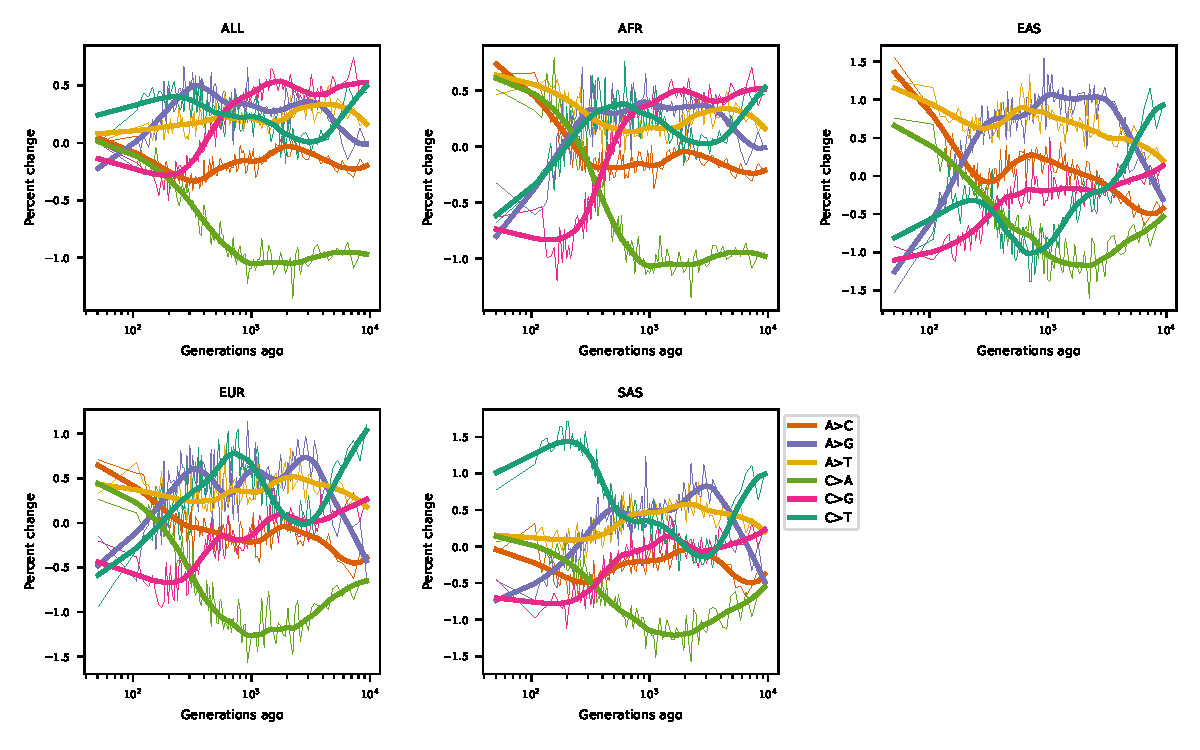
\includegraphics[width=\textwidth]{../plots/spectrum_history.geva.max_age.10000.pdf}
    \caption{
        \textbf{\GEVA-inferred mutation spectrum history.}
        Extending to 10,000 generations in the past, the mutation spectrum history
        from allele ages estimated by \GEVA matches the spectrum history in
        \citet{wang2023human}.
    }
    \label{fig:geva-spectra}
\end{figure}


\begin{figure}[ht!]
    \centering
    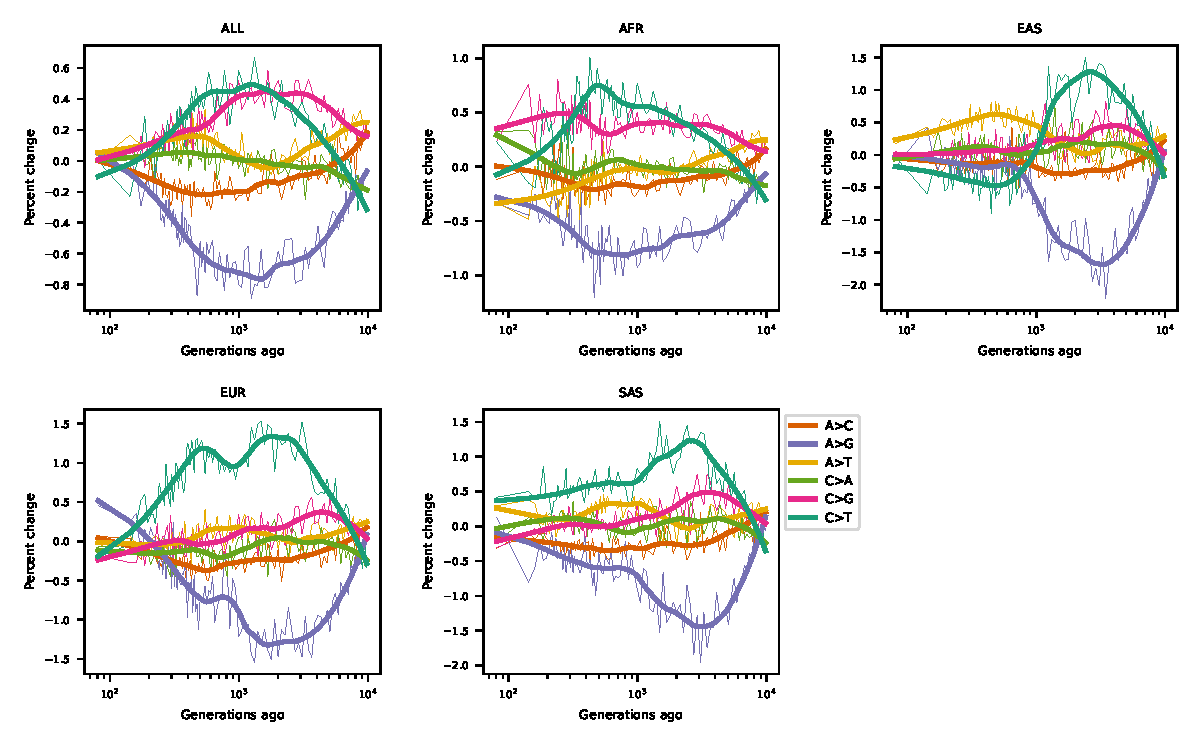
\includegraphics[width=\textwidth]{../plots/spectrum_history.relate.max_age.10000.pdf}
    \caption{
        \textbf{\relate-inferred mutation spectrum history over 10,000 generations.}
    }
    \label{fig:relate-spectra}
\end{figure}


\begin{figure}[ht!]
    \centering
    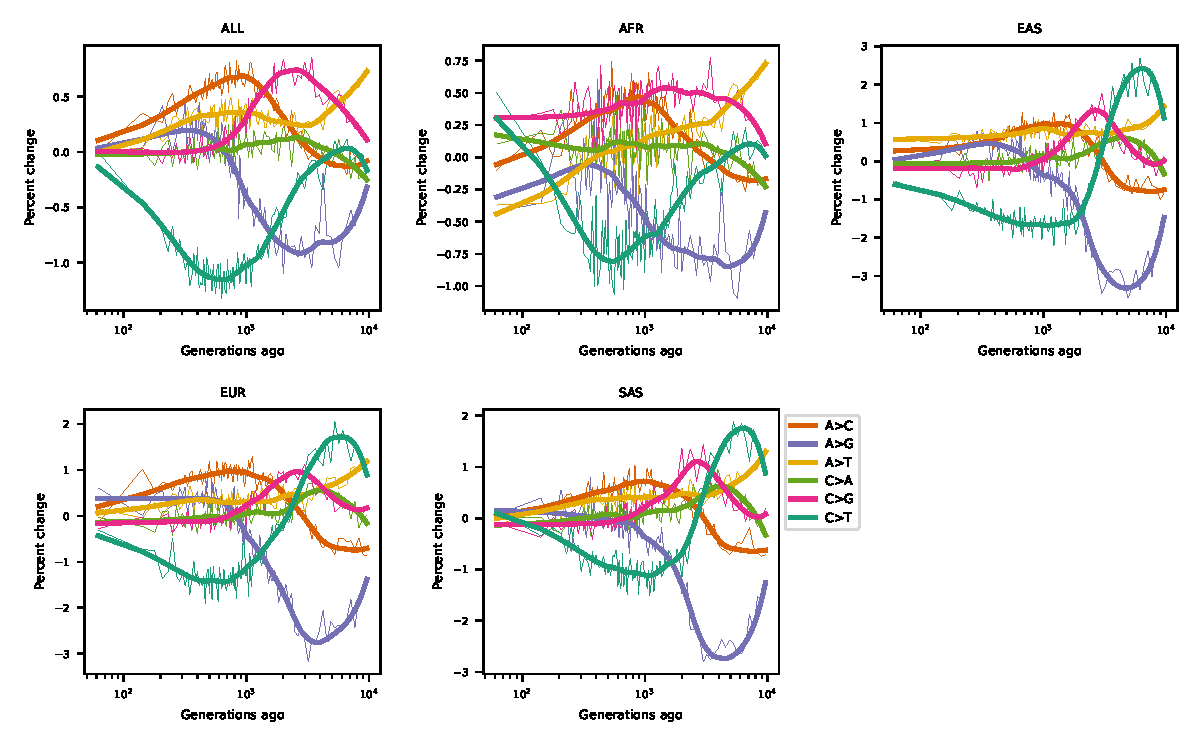
\includegraphics[width=\textwidth]{../plots/spectrum_history.tsdate.max_age.10000.pdf}
    \caption{
        \textbf{\tsdate-inferred mutation spectrum history over 10,000 generations.}
    }
    \label{fig:tsdate-spectra}
\end{figure}


\begin{figure}[ht!]
    \centering
    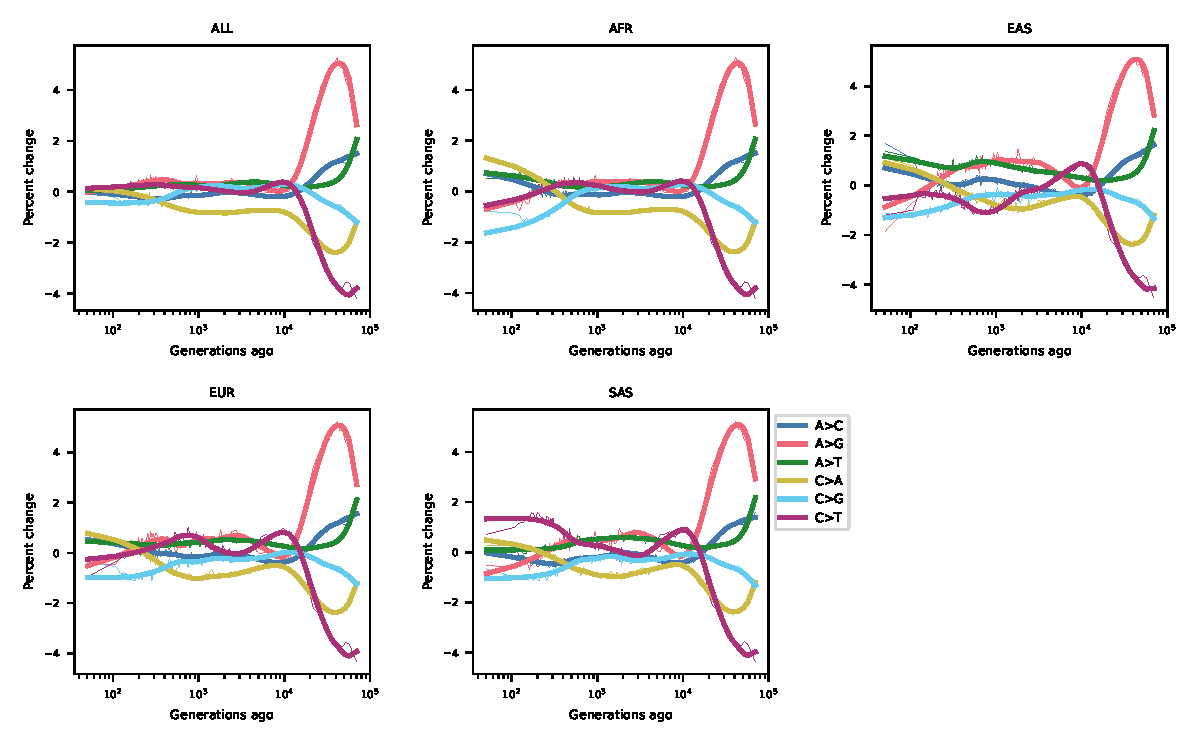
\includegraphics[width=\textwidth]{../plots/spectrum_history.geva.max_age.80000.pdf}
    \caption{
        \textbf{\GEVA-inferred mutation spectrum history, extending to 80,000 generations.}
    }
    \label{fig:geva-spectra-80k}
\end{figure}


\begin{figure}[ht!]
    \centering
    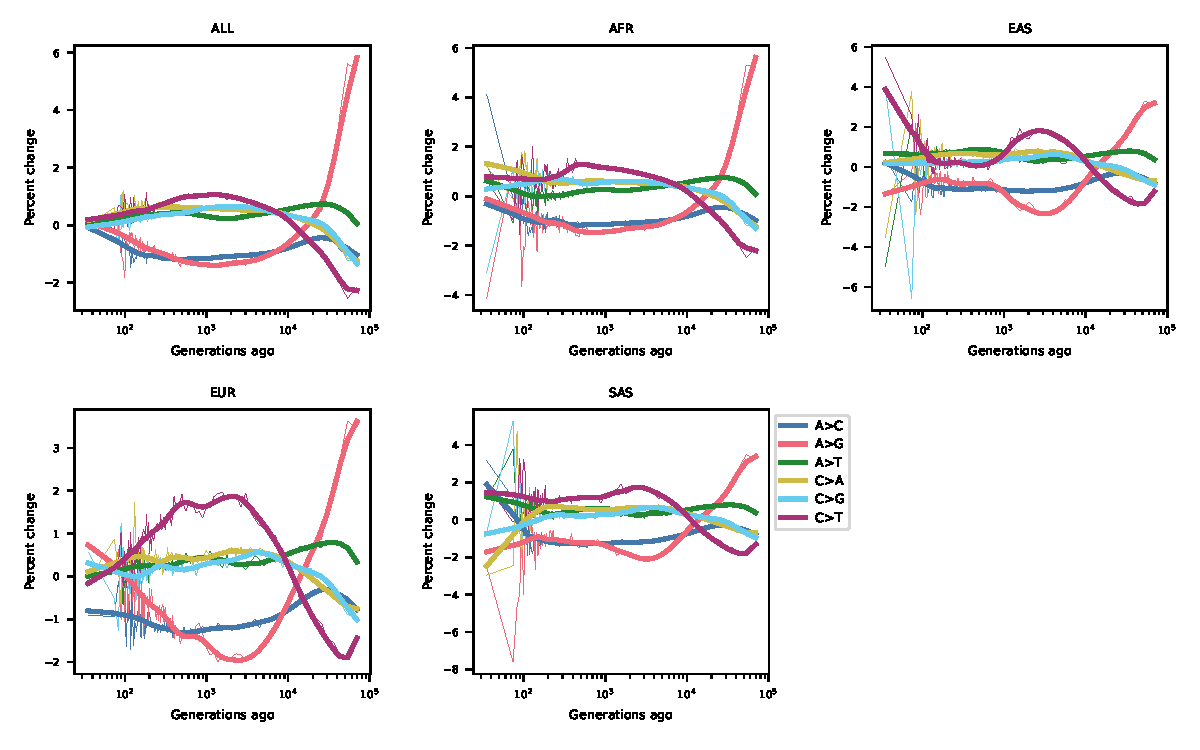
\includegraphics[width=\textwidth]{../plots/spectrum_history.relate.max_age.80000.pdf}
    \caption{
        \textbf{\relate-inferred mutation spectrum history, extending to 80,000 generations.}
    }
    \label{fig:geva-spectra-80k}
\end{figure}


\begin{figure}[ht!]
    \centering
    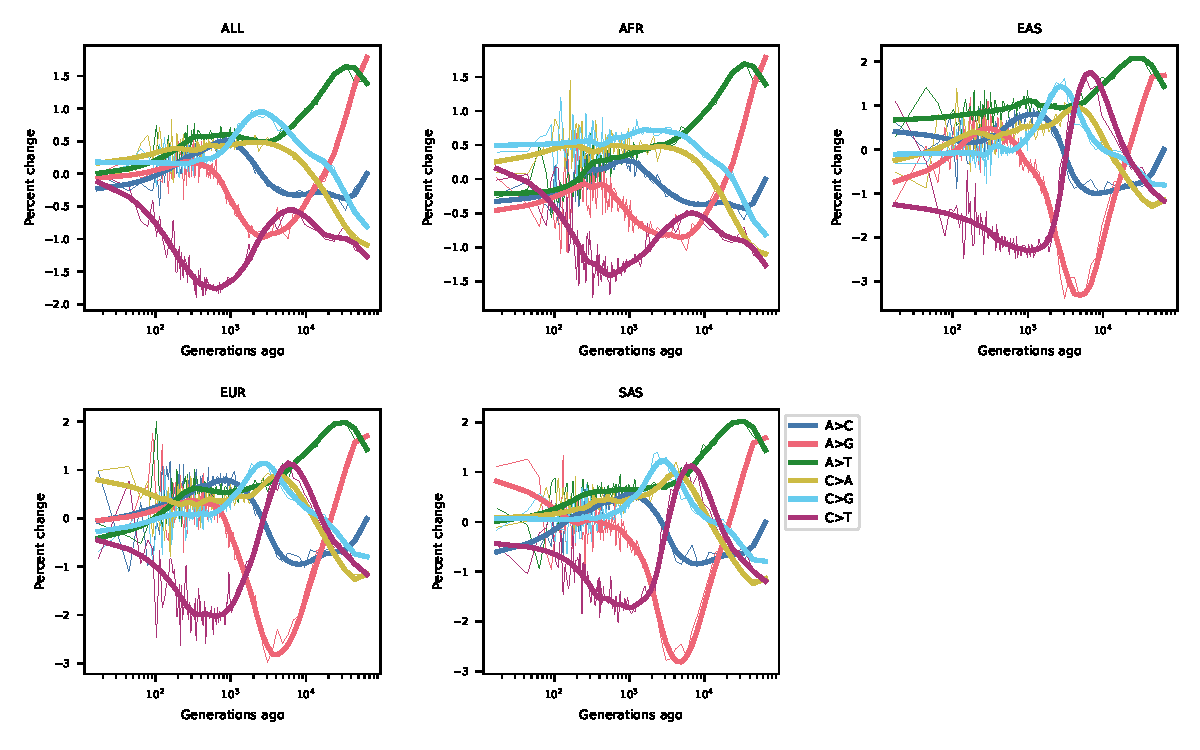
\includegraphics[width=\textwidth]{../plots/spectrum_history.tsdate.max_age.80000.pdf}
    \caption{
        \textbf{\tsdate-inferred mutation spectrum history, extending to 80,000 generations.}
    }
    \label{fig:geva-spectra-80k}
\end{figure}


\begin{figure}[ht!]
    \centering
    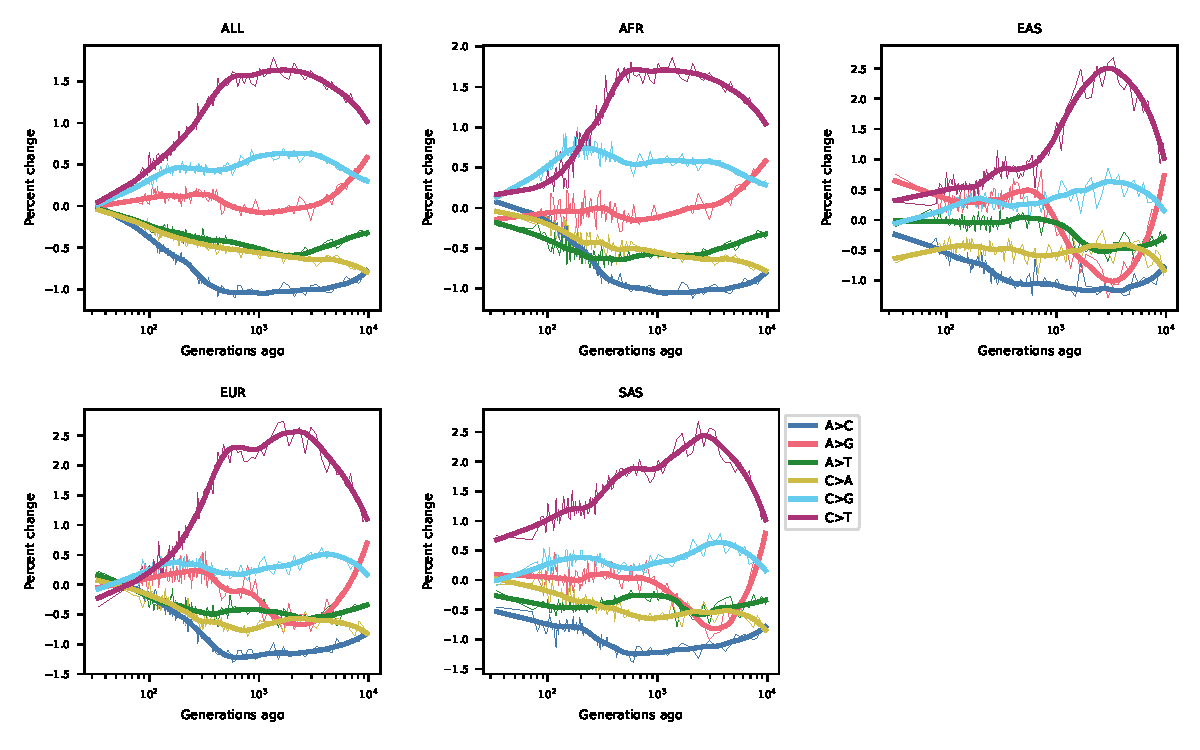
\includegraphics[width=\textwidth]{../plots/spectrum_history.relate.max_age.10000.singletons.pdf}
    \caption{
        \textbf{\relate-inferred mutation spectrum history, including singletons.}
        The inclusion of singletons has only a small effect on the mutation spectrum from
        recent time periods, but a larger effect in older time bins.
        Compare to Figure~\ref{fig:relate-spectra}.
    }
    \label{fig:relate-spectra-singletons}
\end{figure}


\begin{figure}[ht!]
    \centering
    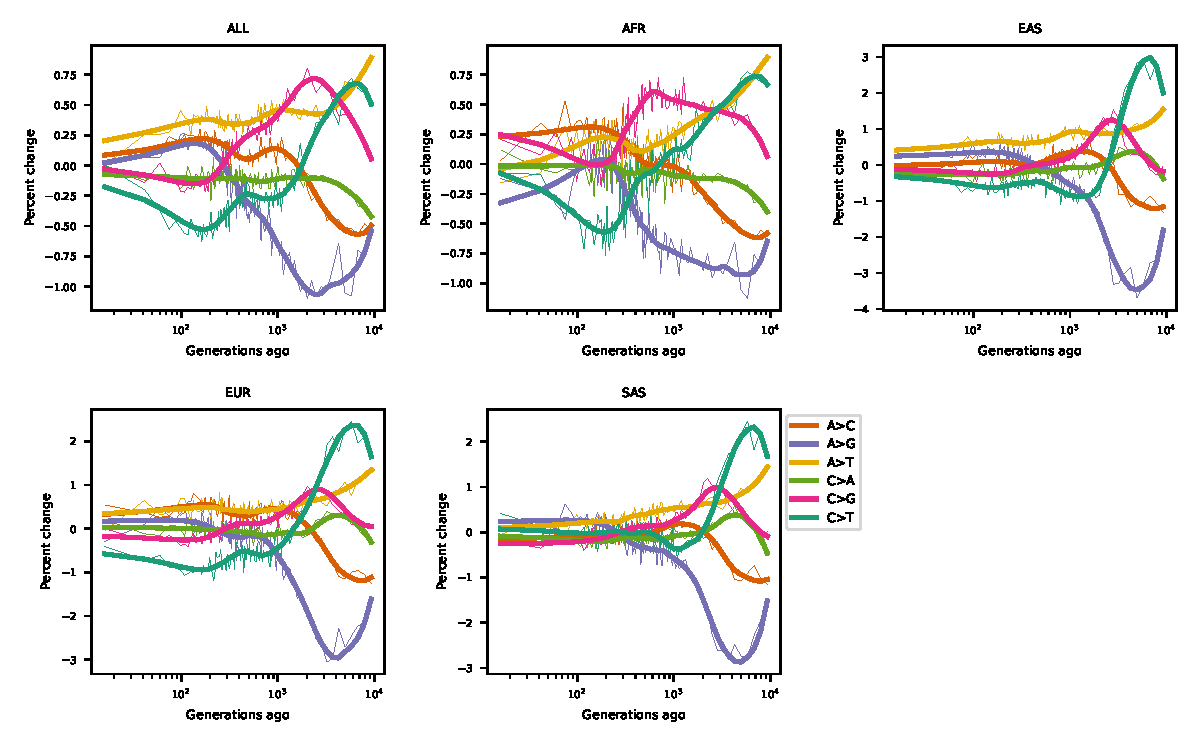
\includegraphics[width=\textwidth]{../plots/spectrum_history.tsdate.max_age.10000.singletons.pdf}
    \caption{
        \textbf{\tsdate-inferred mutation spectrum history, including singletons.}
        The inclusion of singletons using \tsdate does not have as strong of an effect
        on the mutation spectrum history as doing so in \relate
        (Figure~\ref{fig:relate-spectra-singletons}), though still results in some
        qualitative differences from the spectrum history without singletons
        (Figure~\ref{fig:tsdate-spectra}).
    }
    \label{fig:tsdate-spectra-singletons}
\end{figure}


\begin{figure}[ht!]
    \centering
    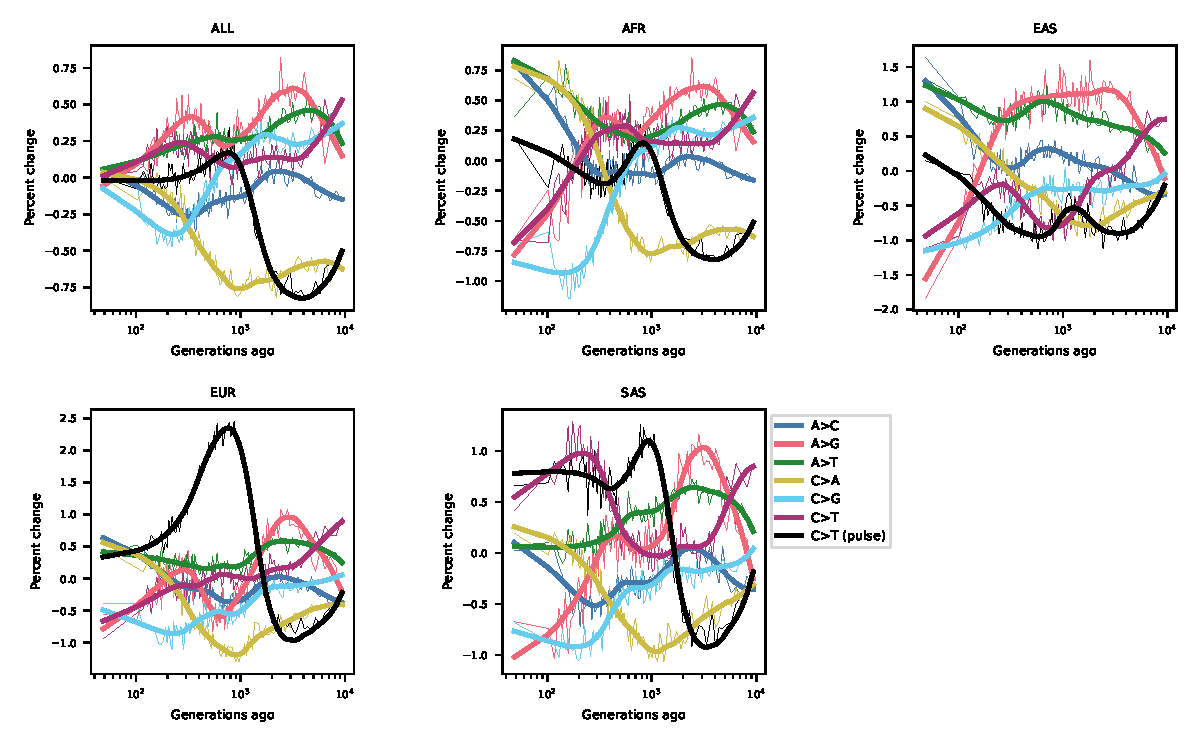
\includegraphics[width=\textwidth]{../plots/spectrum_history.geva.max_age.10000.CtoTpulse.pdf}
    \caption{
        \textbf{\GEVA-inferred mutation spectrum history, including European
            pulse-associated C$\rightarrow$T contexts.}
        \GEVA captures the known pulse of $C\rightarrow T$ mutations among certain
        triplet contexts, in European populations \citep{harris2015evidence}.
    }
    \label{fig:tsdate-spectra-singletons}
\end{figure}


\begin{figure}[ht!]
    \centering
    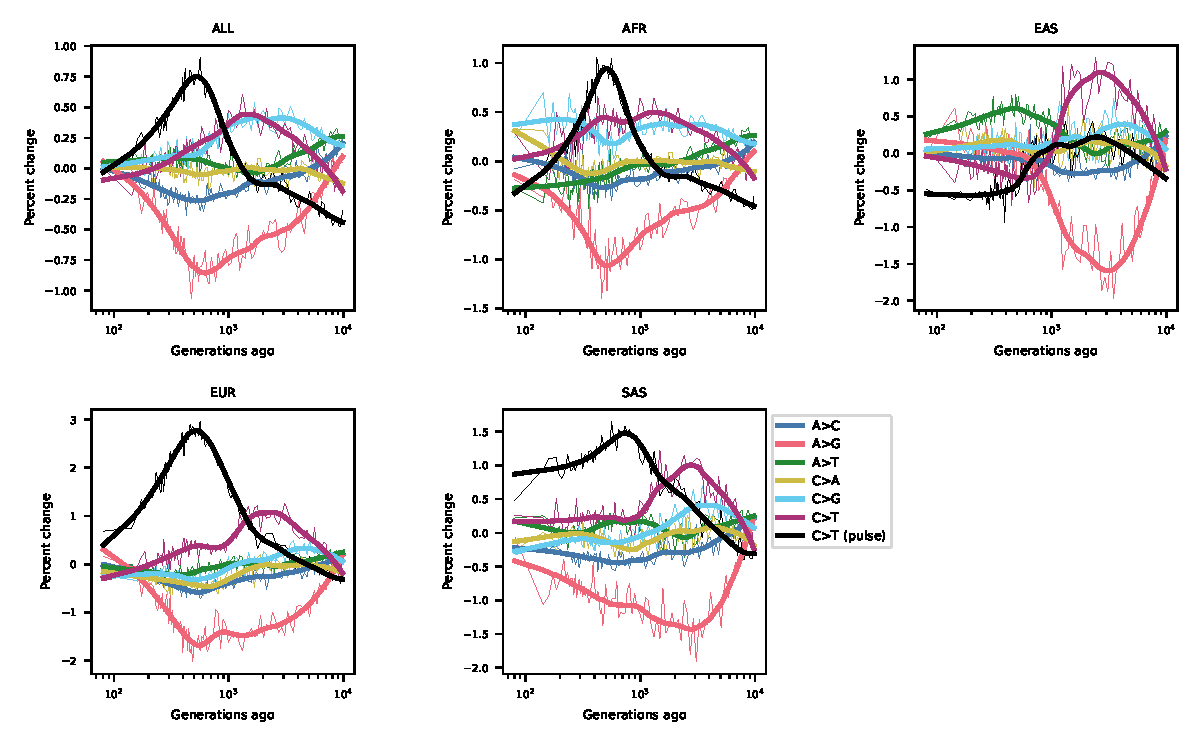
\includegraphics[width=\textwidth]{../plots/spectrum_history.relate.max_age.10000.CtoTpulse.pdf}
    \caption{
        \textbf{\relate-inferred mutation spectrum history, including European
            pulse-associated C$\rightarrow$T contexts.}
        \relate recovers the known pulse of $C\rightarrow T$ mutations in European
        populations, and also finds the same signal in South Asian and African
        populations. South Asians and Europeans have more recent shared ancestry, on
        average, while the signal in African populations could be due to some
        European-related ancestry found in some of the AFR-labeled populations in the
        1KGP (ASW, ACB, and LWK). Note that the scales differ between panels.
    }
    \label{fig:tsdate-spectra-singletons}
\end{figure}


\begin{figure}[ht!]
    \centering
    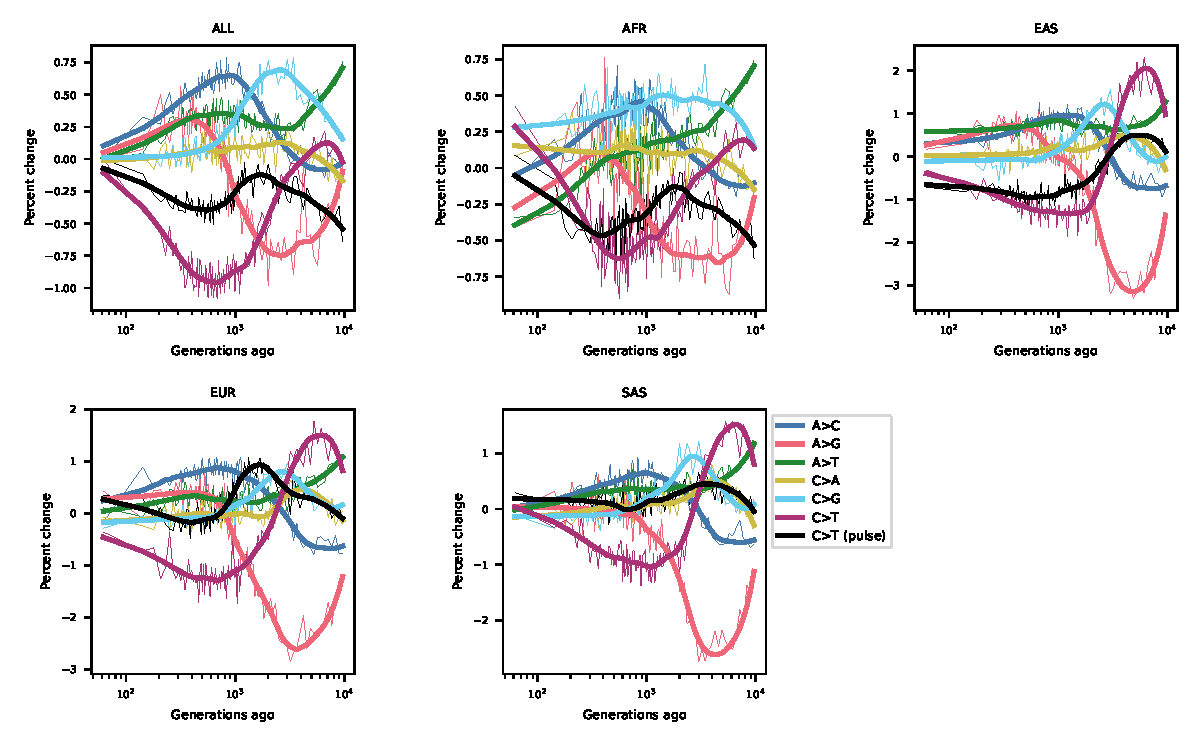
\includegraphics[width=\textwidth]{../plots/spectrum_history.tsdate.max_age.10000.CtoTpulse.pdf}
    \caption{
        \textbf{\tsdate-inferred mutation spectrum history, including European
            pulse-associated C$\rightarrow$T contexts.}
        \tsdate does not pick out the European-related pulse in certain $C\rightarrow T$
        triplet mutation classes.
    }
    \label{fig:tsdate-spectra-singletons}
\end{figure}


\begin{figure}[ht!]
    \centering
    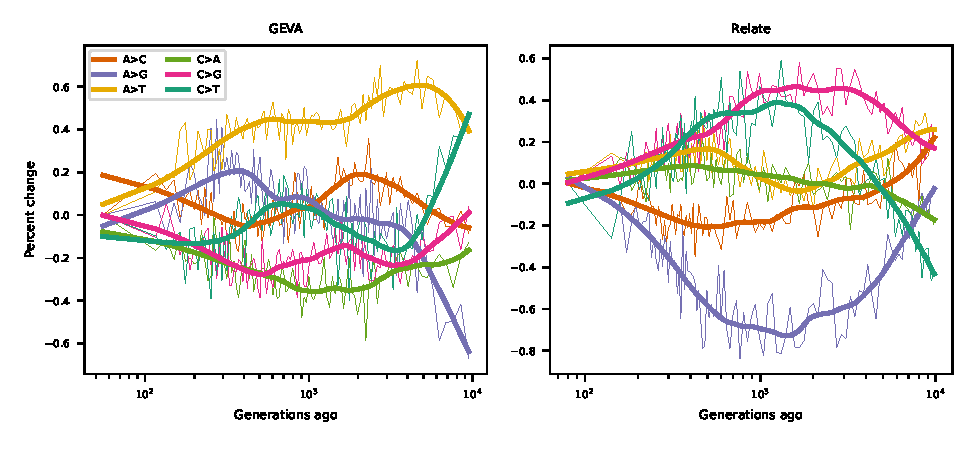
\includegraphics{../plots/overlapping.geva.relate.pdf}
    \caption{
        \textbf{Mutation spectrum histories from mutations that were dated by
        both \GEVA and \relate.}
        Using only mutations that were dated by both \GEVA and \relate, we find
        that the qualitative differences in mutation spectrum histories from
        each method remain. Thus, mutations dated by only one of the two methods
        are unlikely to be driving the differences in mutation spectra between
        methods.
    }
    \label{fig:overlap-spectra}
\end{figure}


\begin{figure}[ht!]
    \centering
    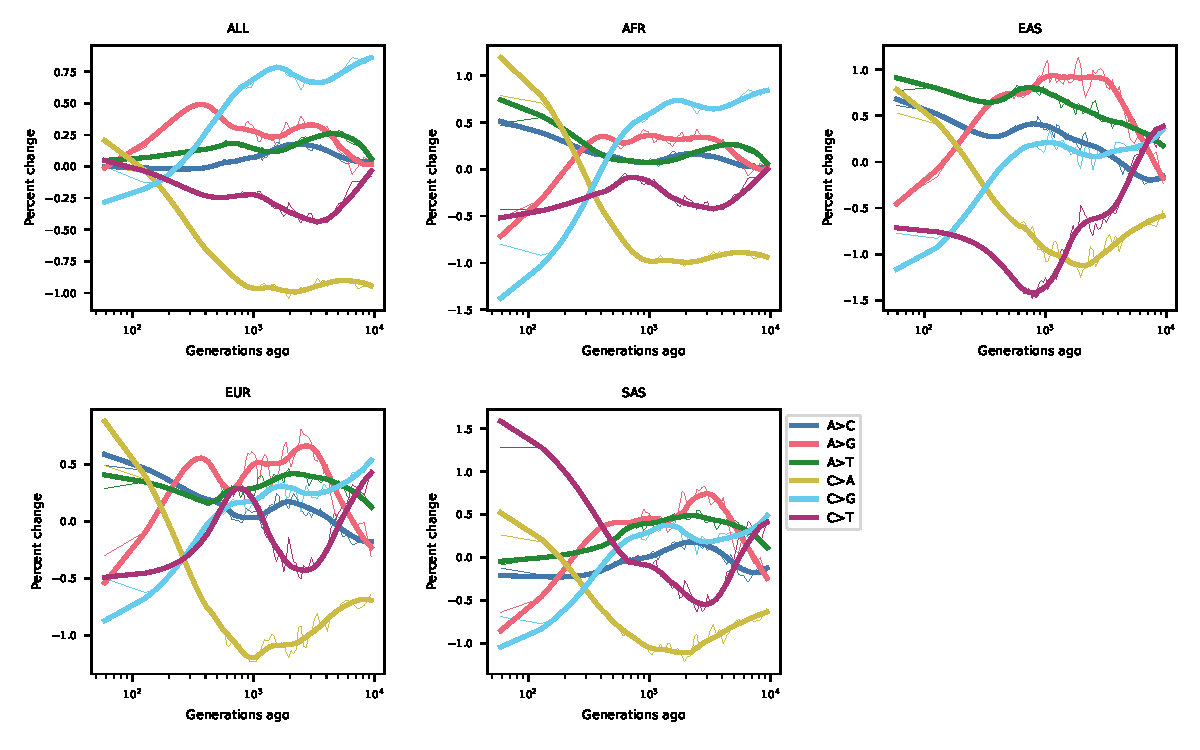
\includegraphics[width=\textwidth]{../plots/spectrum_history.geva.max_age.10000.CI.pdf}
    \caption{
        \textbf{\GEVA-inferred mutation spectrum history, assuming a uniform
        distribution of ages within the 95\% confidence interval.} Compare to
        Figure~\ref{fig:geva-spectra}, which uses the median age estimate
        from \GEVA.
    }
    \label{fig:geva-CI}
\end{figure}


\begin{figure}[ht!]
    \centering
    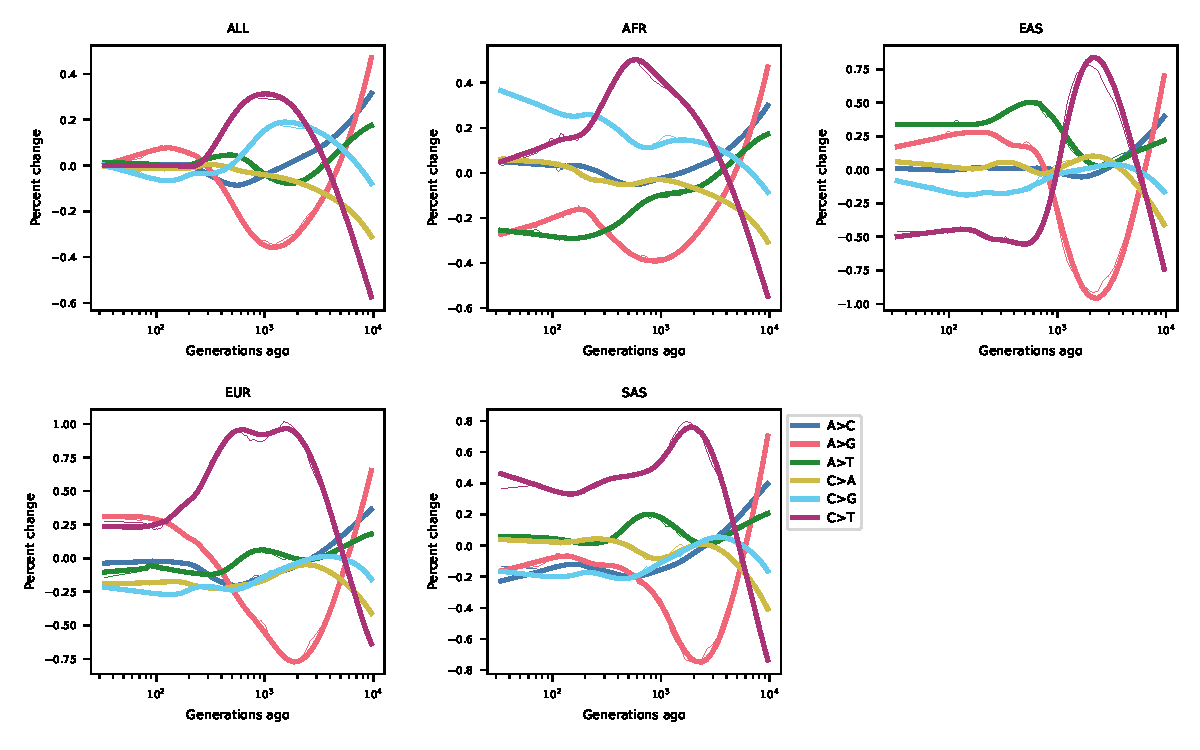
\includegraphics[width=\textwidth]{../plots/spectrum_history.relate.max_age.10000.CI.pdf}
    \caption{
        \textbf{\relate-inferred mutation spectrum history, assuming a uniform
        distribution of ages along a branch.}
        Compare to Figure~\ref{fig:relate-spectra},
        which uses branch midpoints to assign allele ages.
    }
    \label{fig:relate-CI}
\end{figure}



\begin{figure}[ht!]
    \centering
    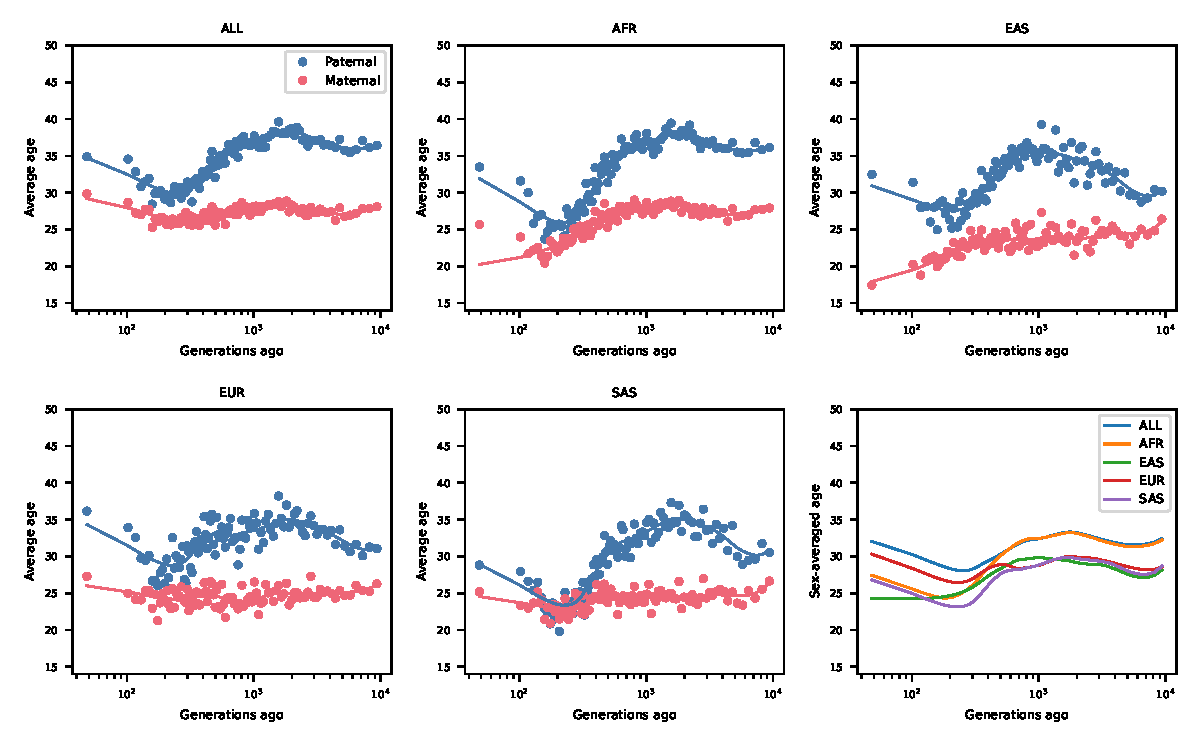
\includegraphics[width=\textwidth]{../plots/inferred_generation_times.DM.geva.max_age.10000.pdf}
    \caption{
        \textbf{\GEVA-inferred generation time histories.}
    }
    \label{fig:geva-gen-times}
\end{figure}

\begin{figure}[ht!]
    \centering
    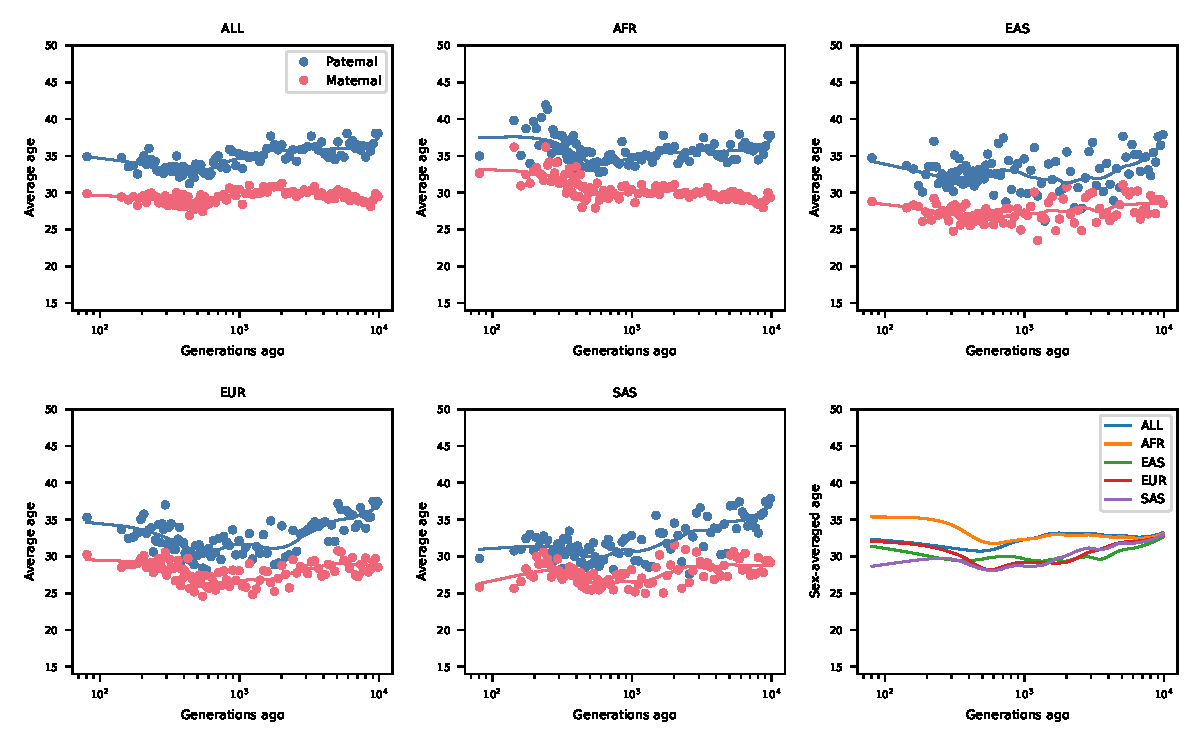
\includegraphics[width=\textwidth]{../plots/inferred_generation_times.DM.relate.max_age.10000.pdf}
    \caption{
        \textbf{\relate-inferred generation time histories.}
    }
    \label{fig:relate-gen-times}
\end{figure}


\begin{figure}[ht!]
    \centering
    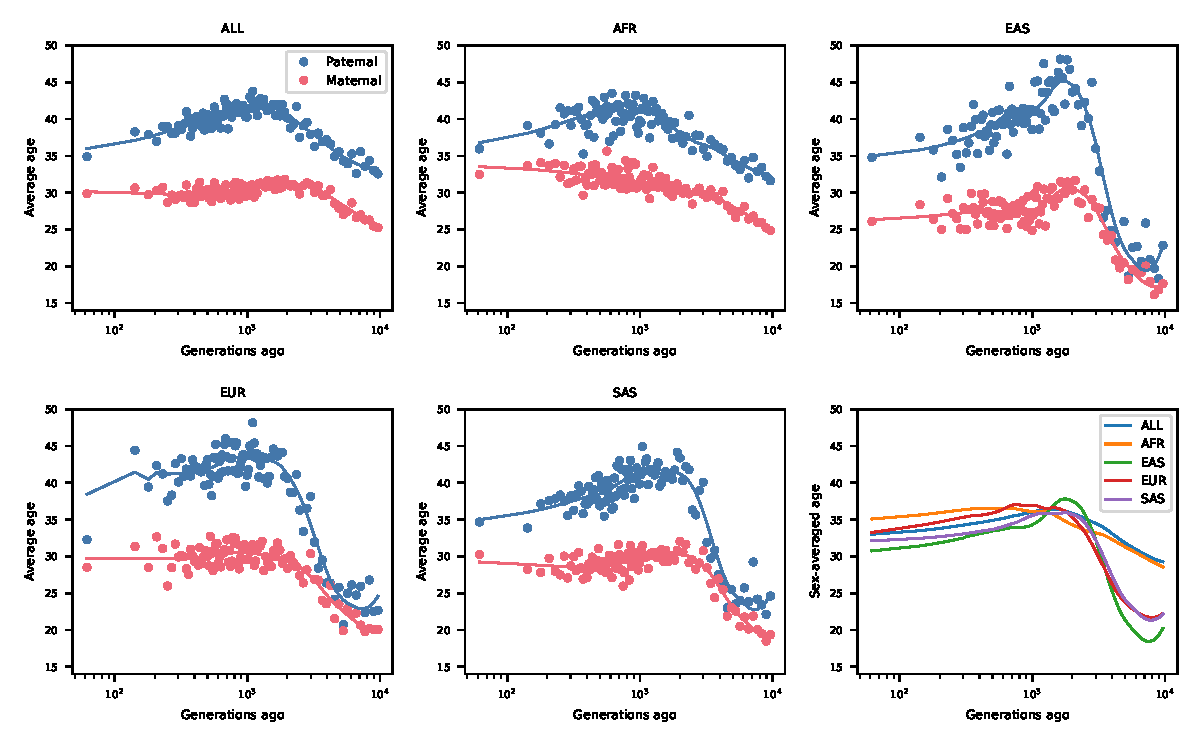
\includegraphics[width=\textwidth]{../plots/inferred_generation_times.DM.tsdate.max_age.10000.pdf}
    \caption{
        \textbf{\tsdate-inferred generation time histories.}
    }
    \label{fig:tsdate-gen-times}
\end{figure}


\begin{figure}[ht!]
    \centering
    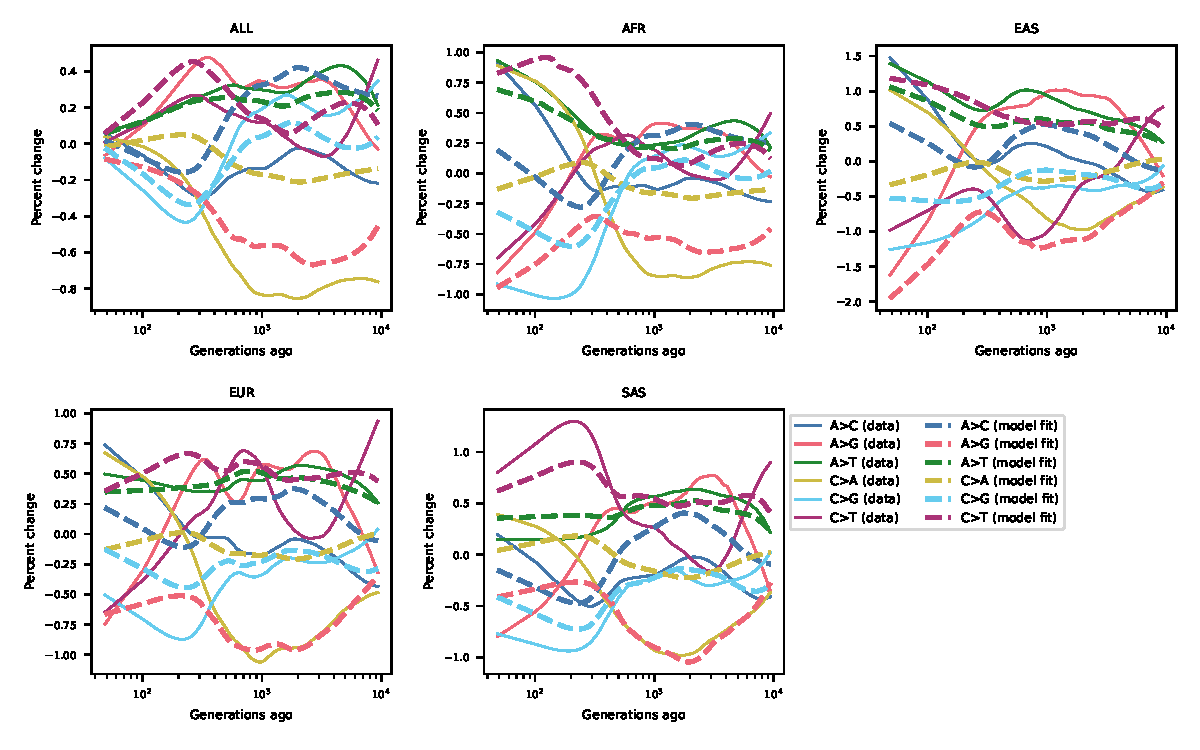
\includegraphics[width=\textwidth]{../plots/goodness-of-fit.DM.geva.max_age.10000.pdf}
    \caption{
        \textbf{Model prediction of mutation spectrum history from
        \GEVA-inferred generation times.}
    }
    \label{fig:geva-fit}
\end{figure}

\begin{figure}[ht!]
    \centering
    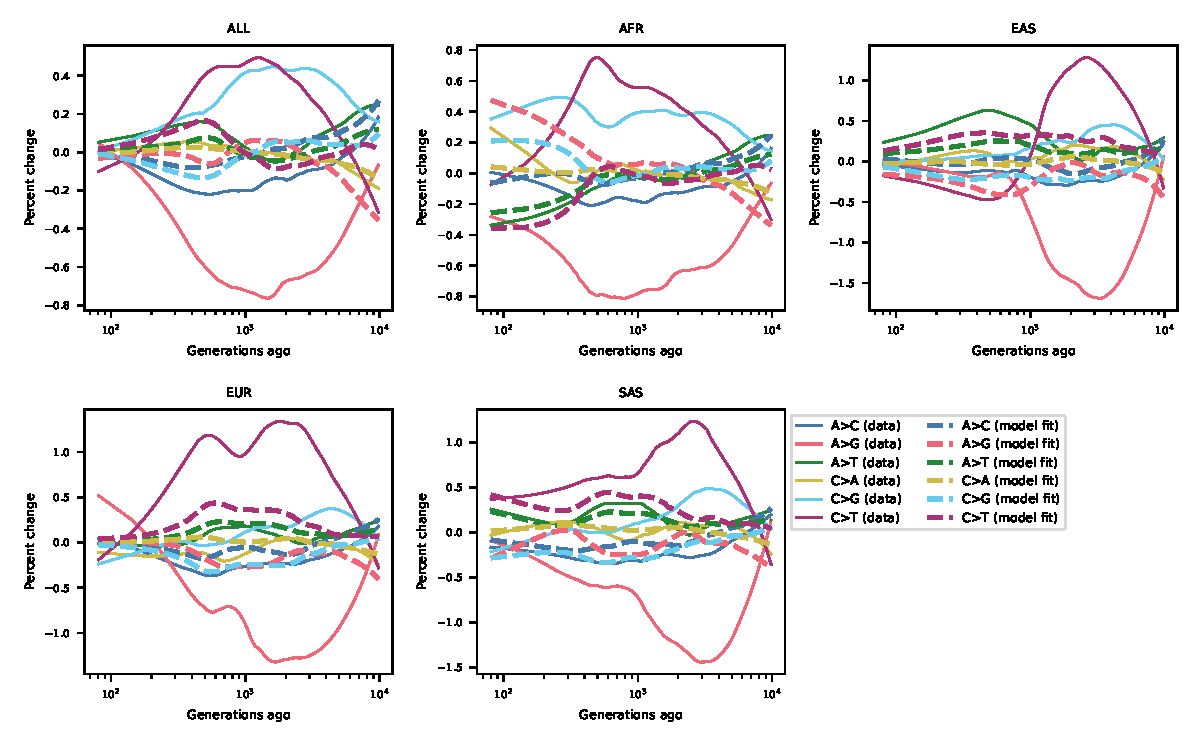
\includegraphics[width=\textwidth]{../plots/goodness-of-fit.DM.relate.max_age.10000.pdf}
    \caption{
        \textbf{Model prediction of mutation spectrum history from
        \relate-inferred generation times.}
    }
    \label{fig:relate-fit}
\end{figure}


\begin{figure}[ht!]
    \centering
    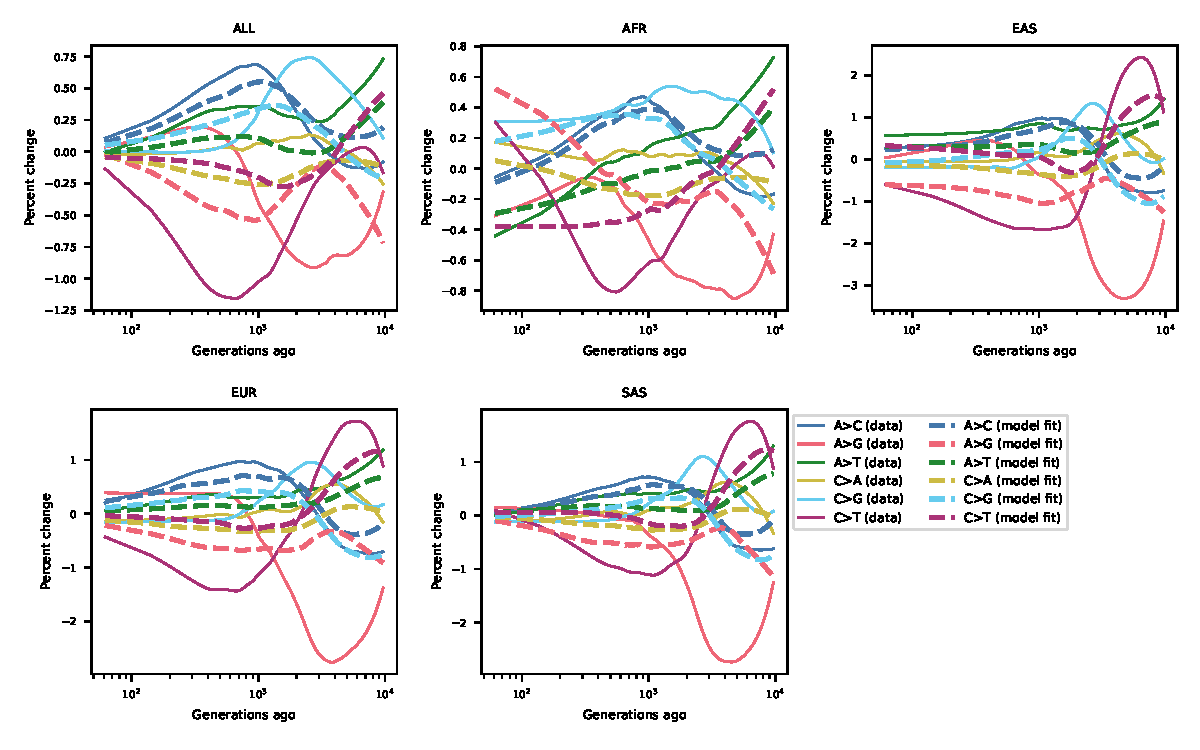
\includegraphics[width=\textwidth]{../plots/goodness-of-fit.DM.tsdate.max_age.10000.pdf}
    \caption{
        \textbf{Model prediction of mutation spectrum history from
        \tsdate-inferred generation times.}
    }
    \label{fig:tsdate-fit}
\end{figure}

\end{document}
